% Supplemental figures (S1, S2, ...)
\renewcommand{\thefigure}{S\arabic{figure}}
\renewcommand{\figurename}{Supplemental Figure}
\setcounter{figure}{0}
\begin{figure}[H]
    \centering
    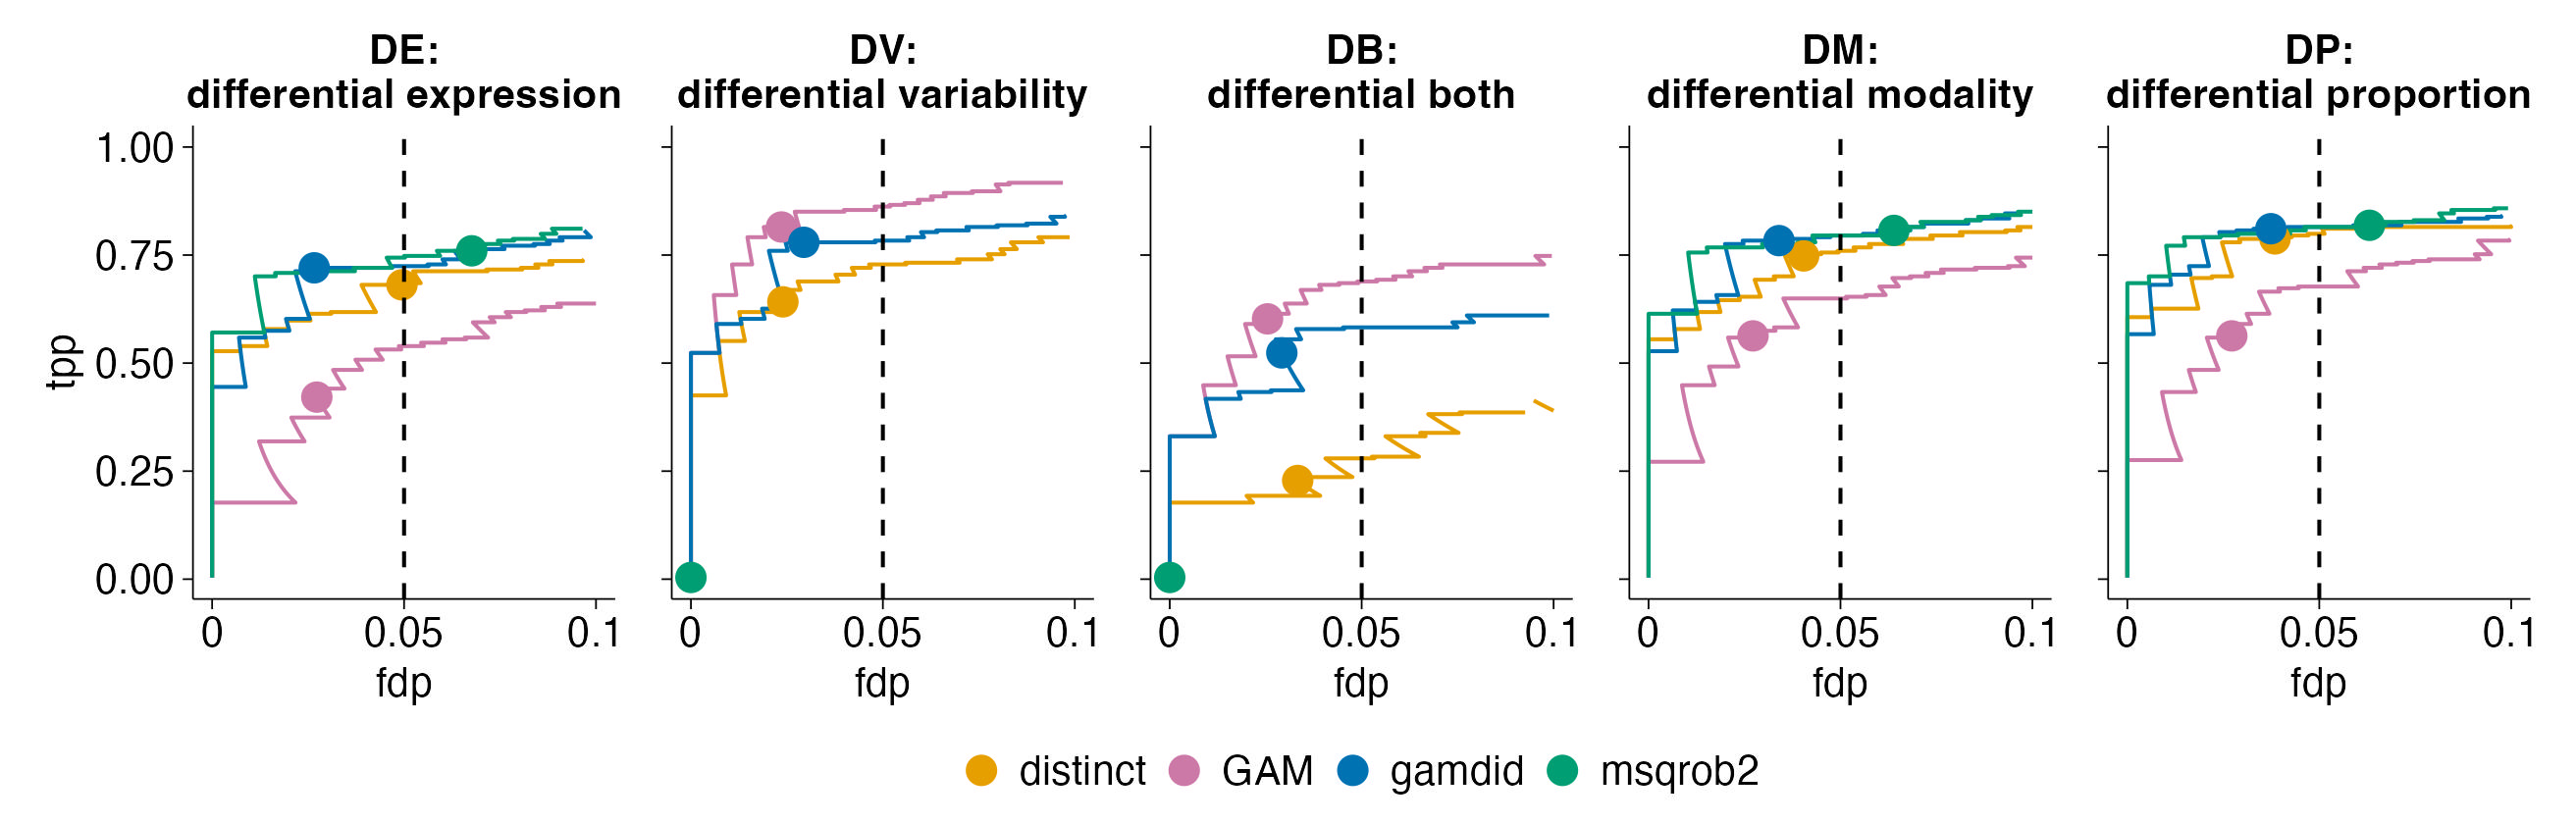
\includegraphics[width=\linewidth]{figs/figS1.jpg}
    \captionsetup{labelfont={bf,small}}
    \caption{\textbf{Performance of gamdid and the standalone GAM method on the Leduc dataset} FDP-TPP curves comparing gamdid, the standalone GAM method, msqrob2 and distinct across the five simulation scenarios, based on the protein-level mock data of the Leduc dataset (755 monocytes). The dots mark the 5\% FDR threshold and the dashed vertical line marks FDP = 0.05. The results are consistent with those for the Petrosius dataset (Figure \ref{fig:sims_petro}): the standalone GAM method outperforms distinct for shape changes (DV, DB) but not when mean shifts are involved (DE, DM, DP), and gamdid combines the strengths of both components while maintaining conservative FDR control. The improvements over distinct are less pronounced than in the Petrosius dataset, which is attributable to the larger sample size: contrary to gamdid, distinct relies on permutation-based inference and suffers from reduced null distribution resolution with fewer observations. DB (differential both) denotes a difference in both modality and component means.}
    \label{fig:sims_leduc}
\end{figure}

\begin{figure}[H]
    \centering
    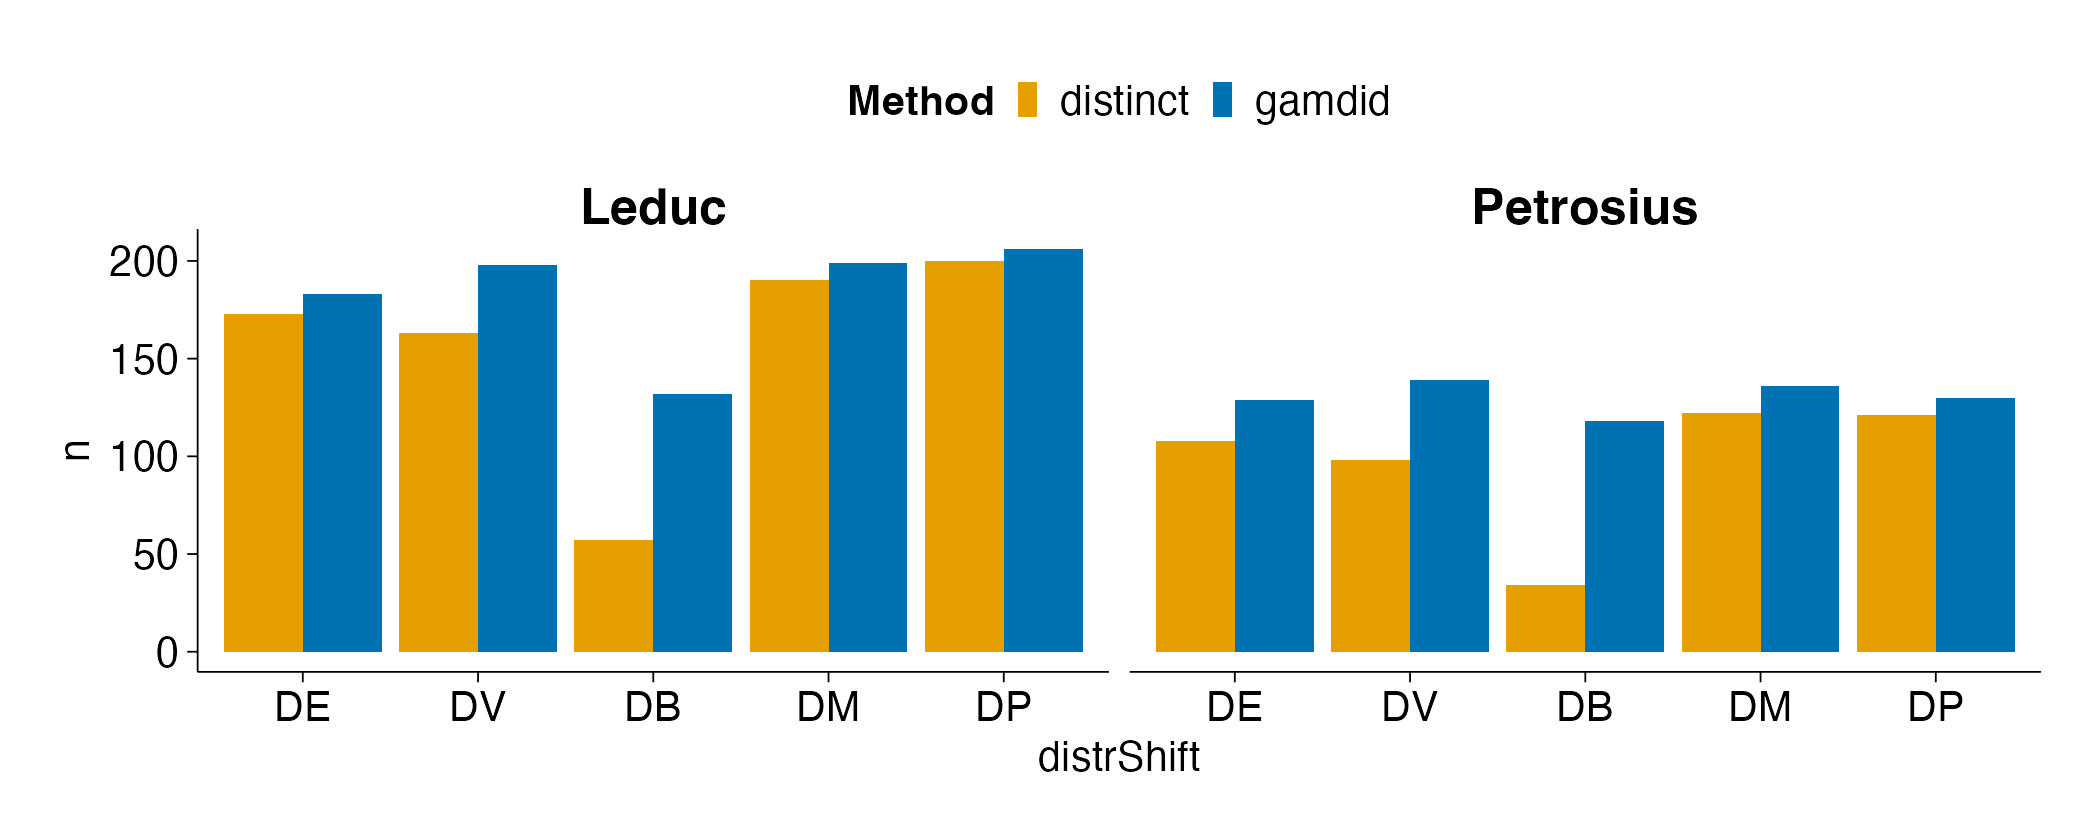
\includegraphics[width=0.85\linewidth]{figs/figS2.jpg}
    \captionsetup{labelfont={bf,small}}
    \caption{\textbf{Absolute true positive counts for gamdid and distinct at 5\% FDR} Bar charts displaying the number of true positives recovered at the nominal 5\% FDR threshold for gamdid and distinct across the five simulation scenarios in the Leduc dataset (left) and the Petrosius dataset (right). gamdid recovers a comparable or greater number of true positives in all scenarios, with the largest absolute gains in the DV and DB scenarios (shape-only differences). The false positive counts (Supplemental Figure \ref{fig:FP}) are similarly low for both methods.}
    \label{fig:TP}
\end{figure}

\begin{figure}[H]
    \centering
    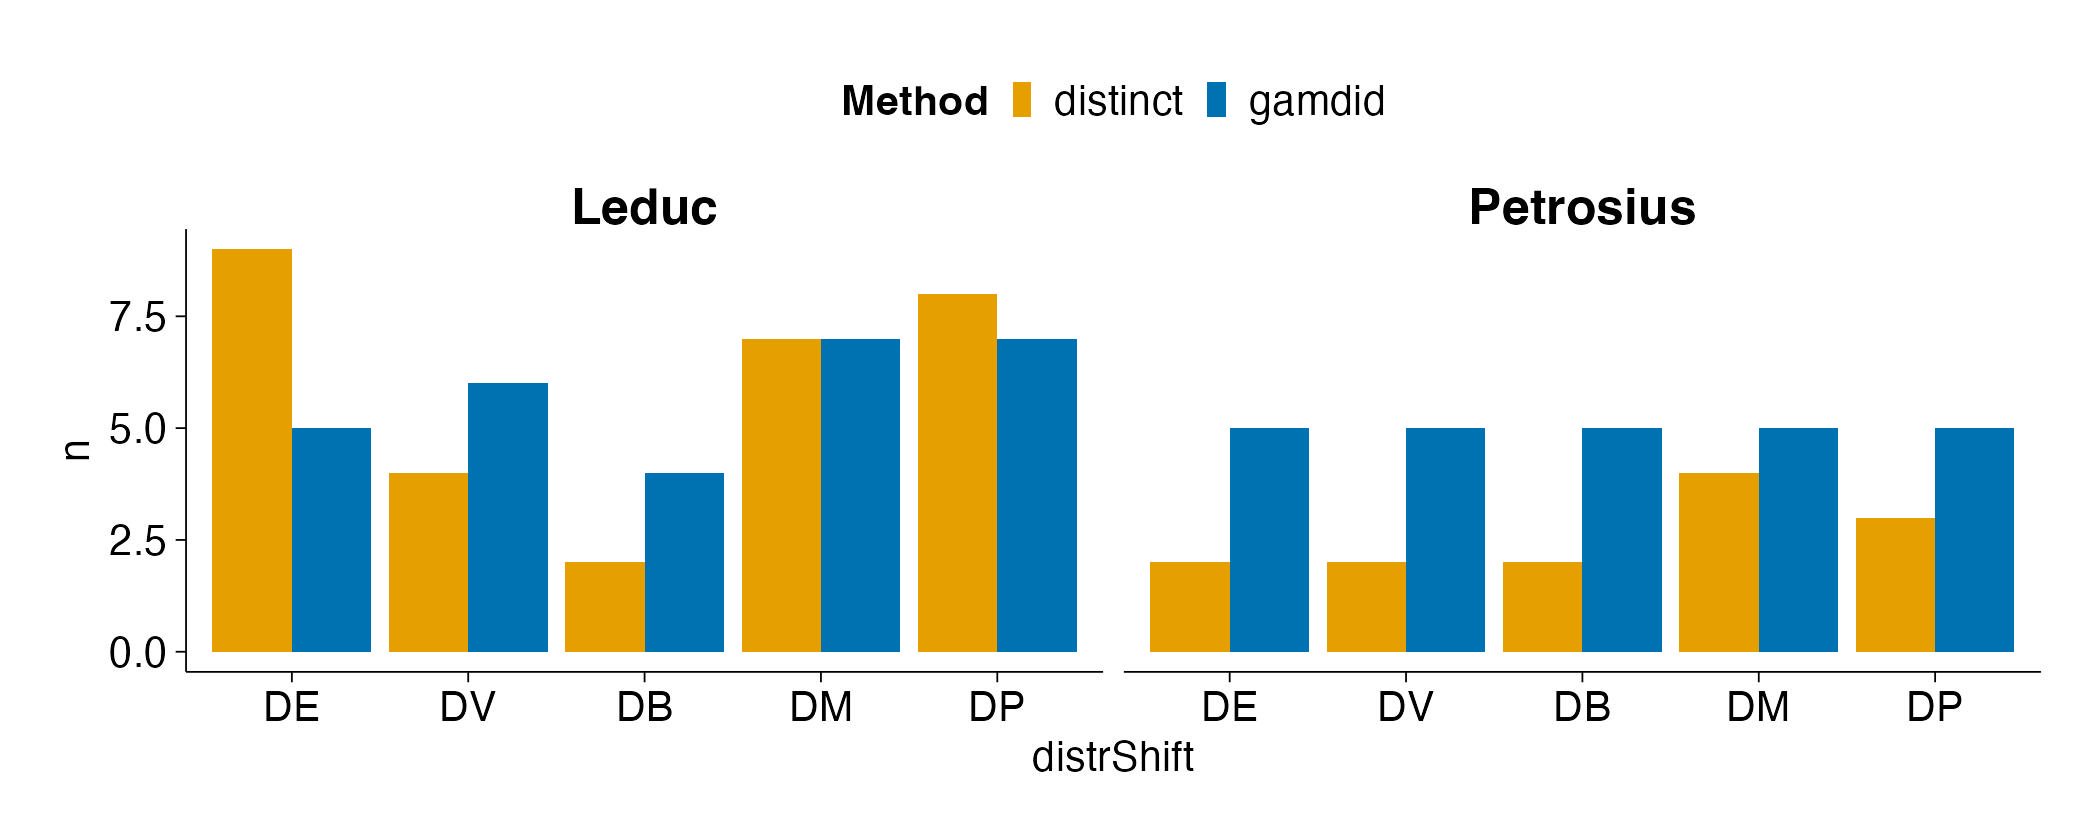
\includegraphics[width=0.85\linewidth]{figs/figS3.jpg}
    \captionsetup{labelfont={bf,small}}
    \caption{\textbf{Absolute false positive counts for gamdid and distinct at 5\% FDR} Bar charts displaying the number of false positives at the nominal 5\% FDR threshold for gamdid and distinct across the five simulation scenarios in the Leduc dataset (left) and the Petrosius dataset (right). Both methods maintain similarly low false positive counts across all scenarios in both datasets, confirming that the gains in true positive recovery demonstrated for gamdid in Supplemental Figure \ref{fig:TP} are not accompanied by inflation of false discoveries.}
    \label{fig:FP}
\end{figure}

\begin{figure}[H]
    \centering
    \includegraphics[width=\linewidth]{figs/figS4.jpg}
    \caption{\textbf{Performance of gamdid on a subsampled Leduc dataset} FDP-TPP curves comparing gamdid and distinct across the five simulation scenarios, based on the protein-level mock data of a subsampled version of the Leduc dataset, in which cells were subsampled such that the average number of non-missing observations per group matched that of the Petrosius dataset. The dots mark the 5\% FDR threshold and the dashed vertical line marks FDP = 0.05. This analysis directly tests whether the more pronounced improvements of gamdid over distinct observed in the Petrosius dataset (see Figure \ref{fig:sims_petro}) are attributable to the smaller sample size. The results support this hypothesis: under reduced sample size, the performance gap between gamdid and distinct increases. distinct likely suffers from reduced null distribution resolution when fewer observations are available. DB (differential both) denotes a difference in both modality and component means.}
    \label{fig:leducsims_gamdid_subsample}
\end{figure}

\begin{figure}[H]
    \centering
    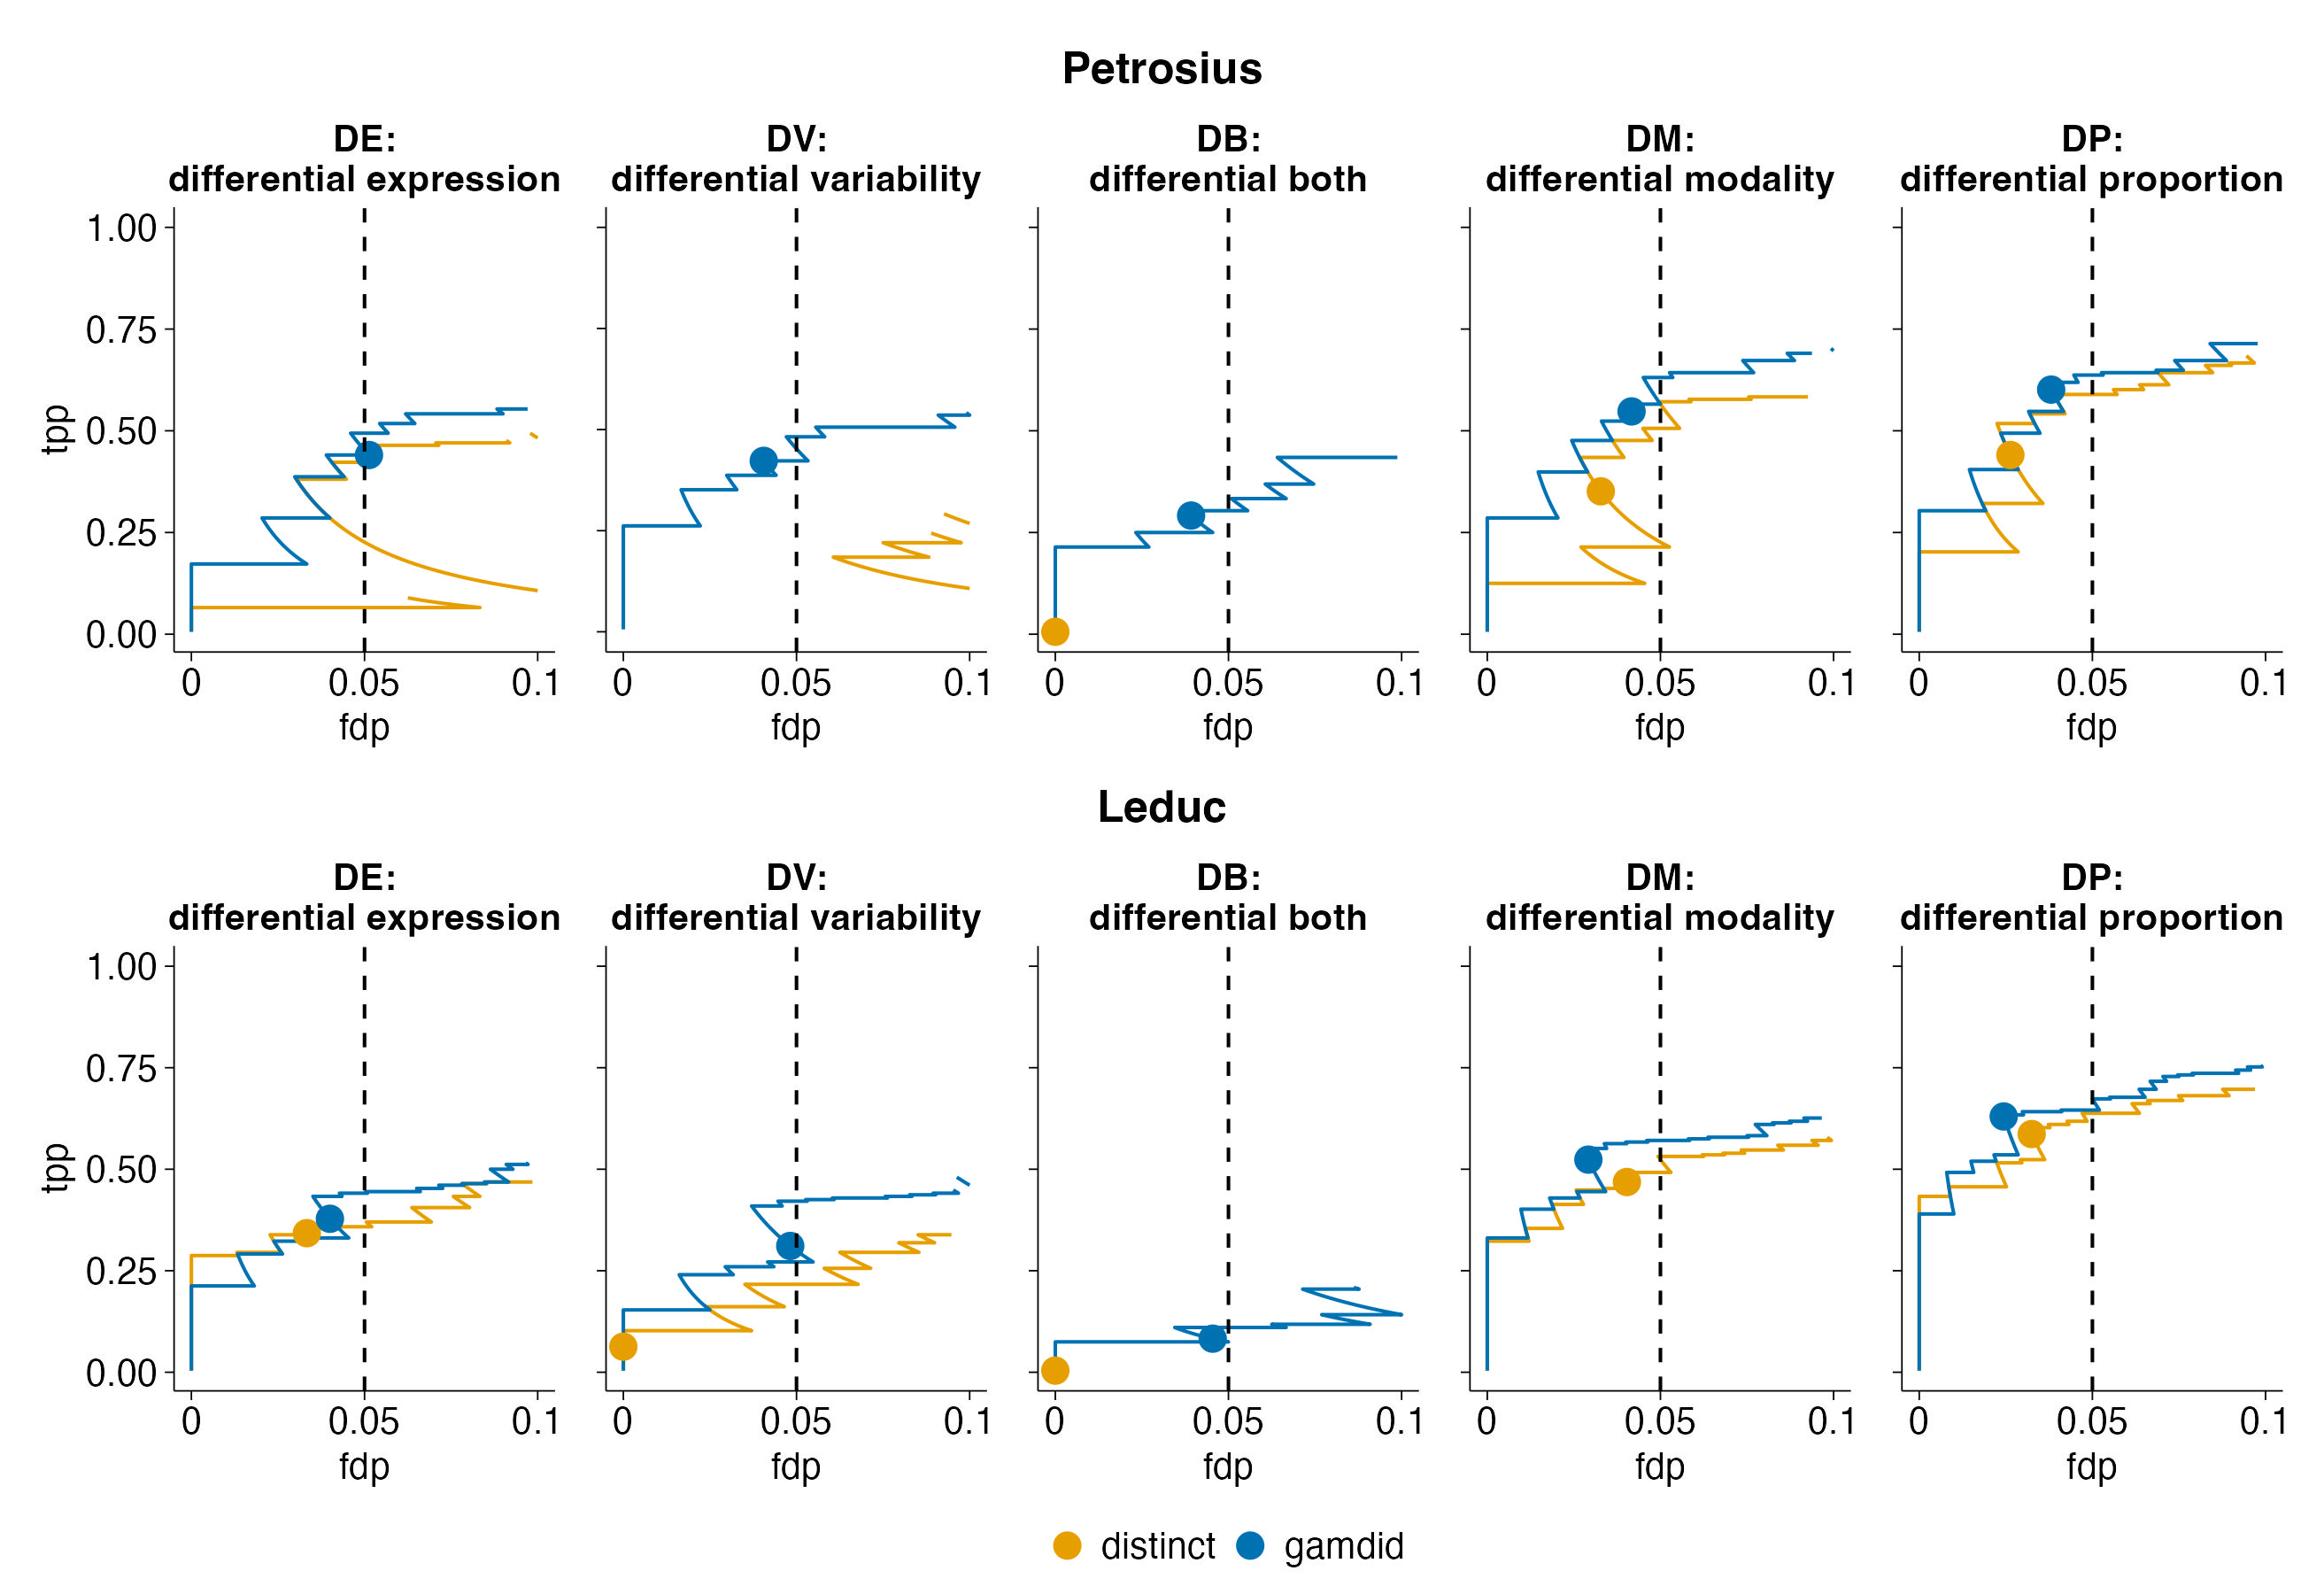
\includegraphics[width=0.85\linewidth]{figs/figS5.jpg}
    \captionsetup{labelfont={bf,small}}
    \caption{\textbf{Performance of gamdid under reduced signal magnitude} FDP-TPP curves comparing gamdid and distinct across the five simulation scenarios, based on the protein-level mock data of the Petrosius dataset (top; 269 m2i cells) and the Leduc dataset (bottom; 755 monocytes), under simulation scenarios with 25\% reduced signal magnitudes (DE: a shift of 30\% instead of 40\% of the feature's standard deviation was used; DV: random Gaussian noise with a standard deviation of 90\% of the feature's standard deviation was added instead of 120\%; DM and DB: a shift of 70\% of the feature's standard deviation was used instead of 90\%, and for DP 75\% instead of 100\%). The dots mark the 5\% FDR threshold and the dashed vertical line marks FDP = 0.05. This analysis assesses whether gamdid's performance advantages are robust to weaker signals that may be encountered in practice. The results are consistent with the original simulations (Figure \ref{fig:sims_petro} and Supplemental Figure \ref{fig:sims_leduc}): gamdid controls the FDR at or below the nominal level and retains its advantages for shape-based distributional changes (DV, DB), while remaining competitive with distinct for scenarios where location shifts are involved. The relative improvements over distinct are more pronounced in the Petrosius dataset, consistent with gamdid's advantage under smaller sample sizes. As expected, the reduced signal does lower the overall power of both methods. DB (differential both) denotes a difference in both modality and component means.}
    \label{fig:leducsims_lower_gamdid}
\end{figure}


\begin{figure}[H]
    \centering
    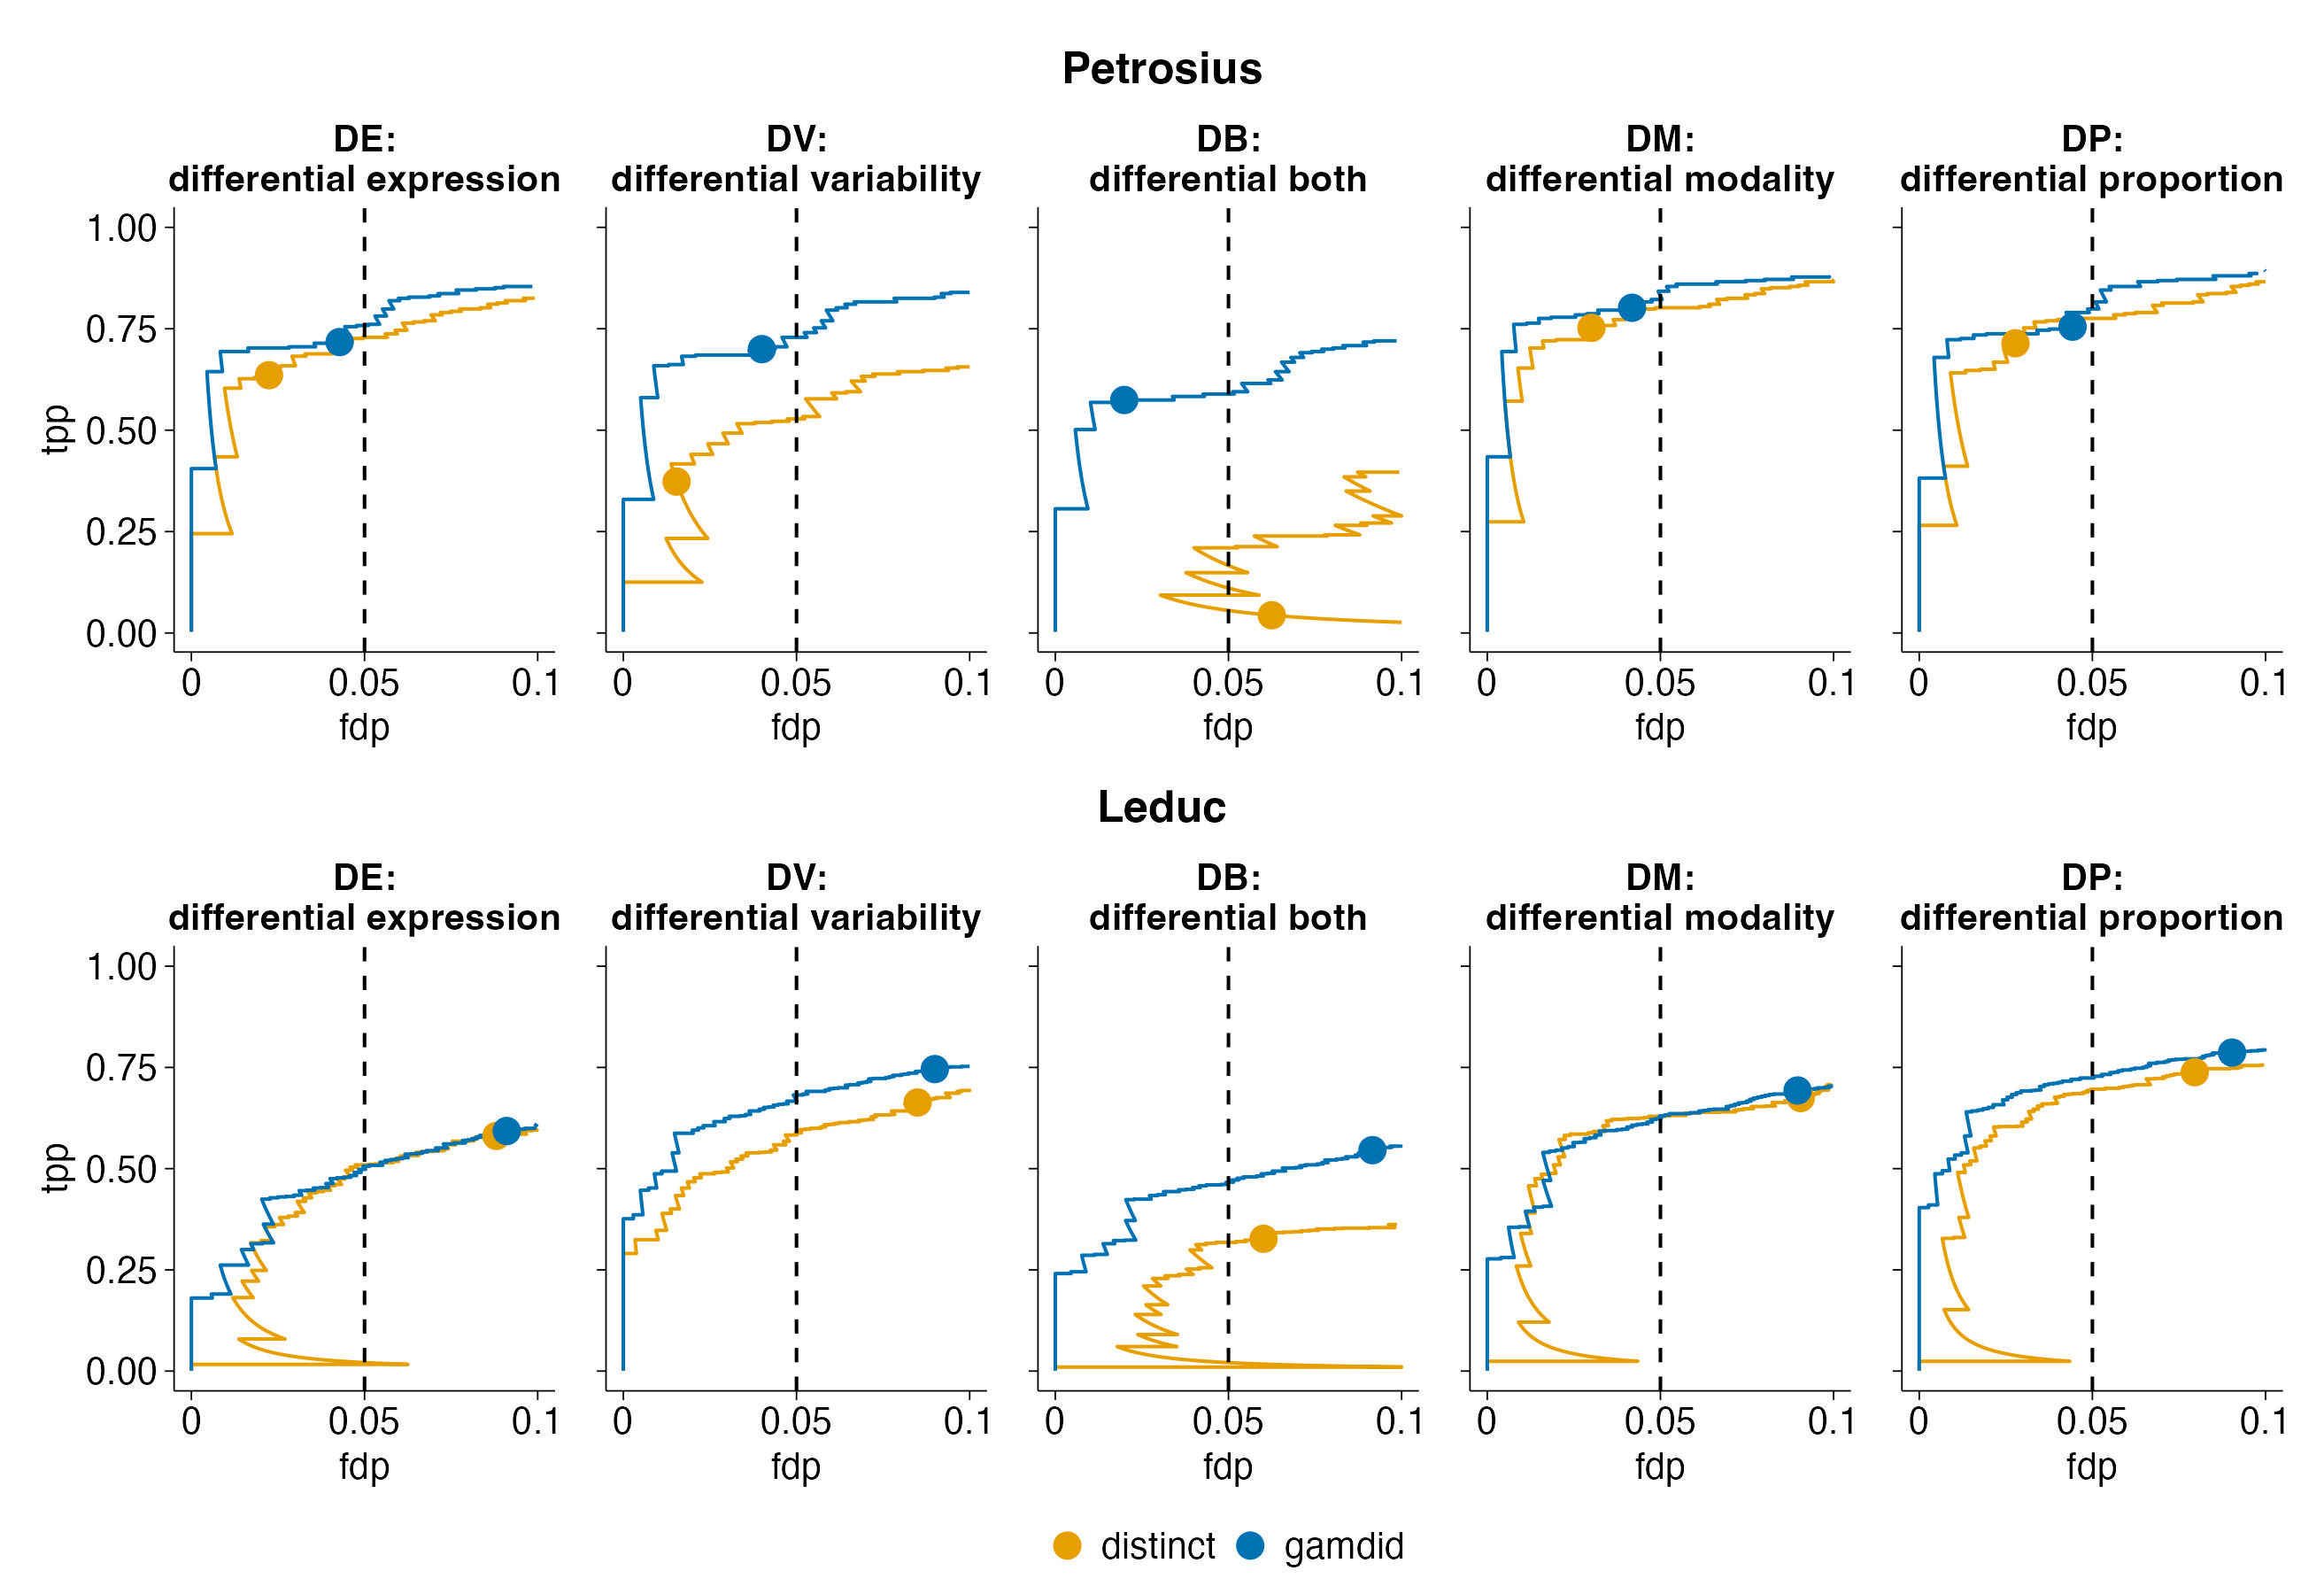
\includegraphics[width=0.85\linewidth]{figs/figS6.jpg}
    \captionsetup{labelfont={bf,small}}
    \caption{\textbf{Performance of gamdid on peptide-level data} FDP-TPP curves comparing gamdid and distinct across the five simulation scenarios, based on the peptide-level mock data of the Petrosius dataset (top; 269 m2i cells) and the Leduc dataset (bottom; 755 monocytes), rather than the protein-level summarized data used in the main analyses. The dots mark the 5\% FDR threshold and the dashed vertical line marks FDP = 0.05. The results are largely consistent with the protein-level findings (Figure \ref{fig:sims_petro} and Supplemental Figure \ref{fig:sims_leduc}), and gamdid retains its performance advantages. In the Leduc dataset, the observed FDP at the 5\% FDR threshold for both methods suggests that the nominal FDR is not well controlled at the peptide level, which reflects a well-known challenge in peptide-level data: multiple peptides mapping to the same protein are correlated. In the Petrosius dataset, gamdid controls the FDR at the peptide level. Despite the liberal FDR control in the Leduc dataset, gamdid provides a flexible and applicable framework across all processing levels of proteomics data. DB (differential both) denotes a difference in both modality and component means.}
    \label{fig:leducsims_pep}
\end{figure}


\begin{figure}[H]
    \centering
    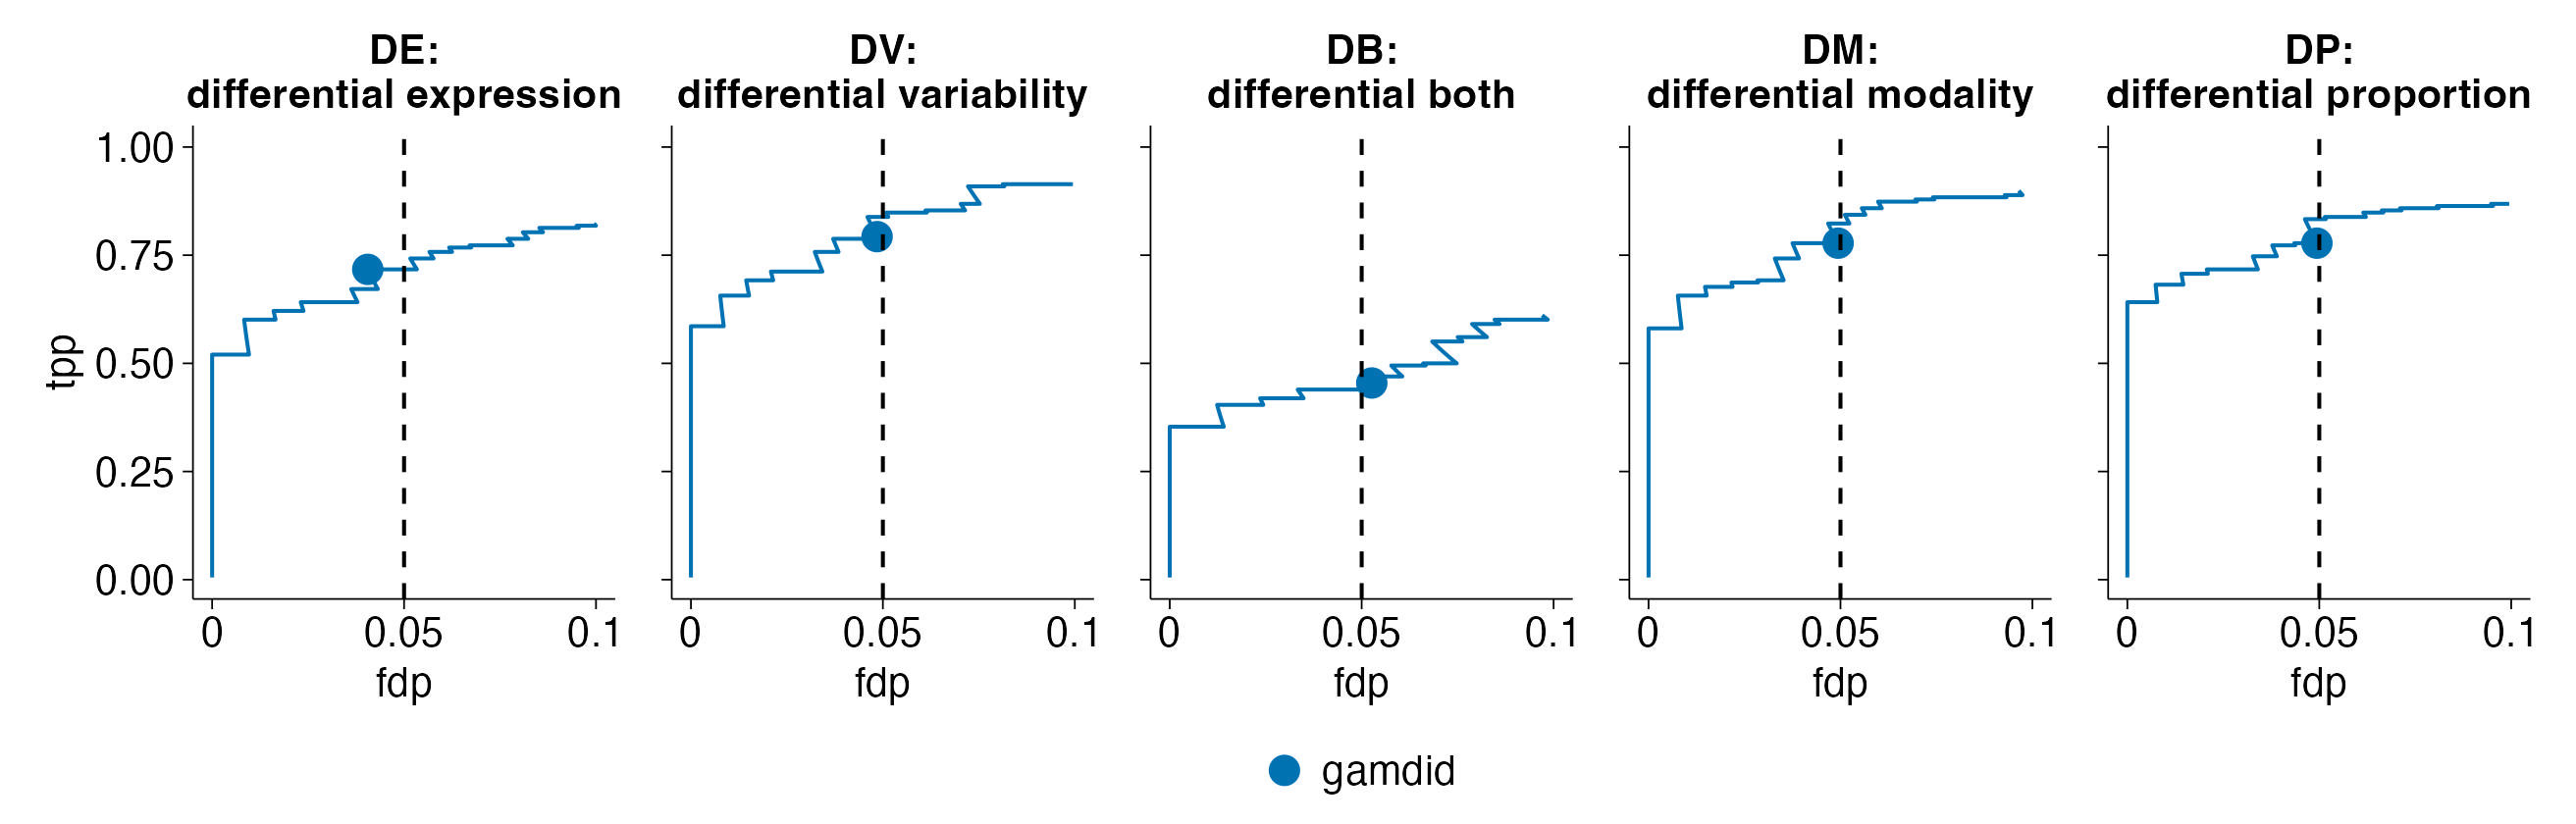
\includegraphics[width=\linewidth]{figs/figS7.jpg}
    \caption{\textbf{Performance of the gamdid omnibus test in a three-group simulation} FDP-TPP curves for gamdid's omnibus test across the five simulation scenarios, based on the protein-level mock data of the Leduc dataset (755 monocytes). Cells were randomly assigned to three mock groups (A, B, C), with distributional signal introduced in group B under the same five simulation scenarios as in the two-group analyses. No competing DD method currently supports multi-group omnibus testing, so no benchmark comparison is possible here; these curves demonstrate gamdid's standalone performance in this setting. The dots mark the 5\% FDR threshold and the dashed vertical line marks FDP = 0.05. Notably, the three-group omnibus test achieves higher power than the corresponding two-group comparisons in Supplemental Figure \ref{fig:sims_leduc}. DB (differential both) denotes a difference in both modality and component means.}
    \label{fig:leduc_threegroup}
\end{figure}




\clearpage
\begin{figure}[H]
    \centering
    \includegraphics[width=0.85\linewidth,height=0.75\textheight,keepaspectratio]{figs/figS8.jpg}
    \captionsetup{labelfont={bf,small}}
    \caption{\textbf{gamdid visualizations for features detected only by msqrob2 or only by distinct in the spike-in case study} The output of gamdid's visFit function for two of the four features flagged as significant exclusively by msqrob2 (\textbf{A}, \textbf{B}) and the two features flagged as significant exclusively by distinct (\textbf{C}, \textbf{D}). Each panel shows the mock comparison (top), in which the groups show no distributional difference, the comparison after spiking 10\% of the 697 sub-cluster A melanoma cells (69 cells) into group Y (middle), and a boxplot indicating where the spike-in melanoma cells are located (bottom). \textbf{A--B}: After spike-in, a weak mean shift appears, but no differential region is found by gamdid (no gray shading). This illustrates a feature type where msqrob2's dedicated sensitivity for mean shifts gives it a slight edge over gamdid. \textbf{C}: After spike-in, the melanoma cells add a heavier left tail to the distribution of group Y, but no differential region is found by gamdid (no gray shading). Here, distinct's ECDF-based approach accumulates sufficient evidence to reach significance, while gamdid's local density approach does not identify a sufficiently concentrated differential region. \textbf{D}: After spike-in, the density of group Y shifts in the right tail, and gamdid's difference smoother identifies a differential region (gray shading), despite the FDR-adjusted p-value being non-significant (gamdid FDR-adjusted p-value = 0.090).}
    \label{fig:msqrob_distinct_only}
\end{figure}
\clearpage




\begin{figure}[H]
    \centering
    \includegraphics[width=0.425\linewidth]{figs/figS9.jpg}
    \caption{\textbf{Computational efficiency of gamdid and distinct}
    Mean runtime for gamdid and distinct on the spike-in case study dataset
    (1316 features, 824 cells), each run on a single core and averaged
    across ten independent runs. gamdid completed in 16 seconds on average,
    whereas distinct required 256 seconds, corresponding to a more than
    fifteen-fold speedup.}
  \label{fig:runtime}
\end{figure}
